\footnotesize
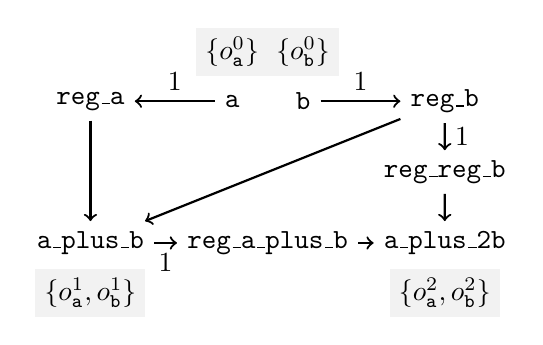
\begin{tikzpicture}[scale=.9,thick]
    \node (a) at (2, 0) {$\textpurple{\mathtt{a}}$};
    \node (b) at (3, 0) {$\textpurple{\mathtt{b}}$};
    \node (ra) at (0, 0) {$\mathtt{reg\_a}$};
    \node (rb) at (5, 0) {$\mathtt{reg\_b}$};
    \node (rrb) at (5, -1) {$\mathtt{reg\_reg\_b}$};
    \node (ab) at (0, -2) {$\textblue{\mathtt{a\_plus\_b}}$};
    \node (rab) at (2.5, -2) {$\mathtt{reg\_a\_plus\_b}$};
    \node (a2b) at (5, -2) {$\textblue{\mathtt{a\_plus\_2b}}$};

    \draw [->] (a) --node[above]{$1$} (ra);
    \draw [->] (ra) -- (ab);
    \draw [->] (rb) -- (ab);
    \draw [->] (b) --node[above]{$1$} (rb);
    \draw [->] (rb) --node[right]{$1$} (rrb);
    \draw [->] (ab) --node[below]{$1$} (rab);
    \draw [->] (rab) -- (a2b);
    \draw [->] (rrb) -- (a2b);

    \node[fill=gray!10] at (2, .7) {$\{o_{\mathtt{a}}^0\}$};
    \node[fill=gray!10] at (3, .7) {$\{o_{\mathtt{b}}^0\}$};

    \node[fill=gray!10] at (0, -2.7) {$\{o_{\mathtt{a}}^1, o_{\mathtt{b}}^1\}$};
    \node[fill=gray!10] at (5, -2.7) {$\{o_{\mathtt{a}}^2, o_{\mathtt{b}}^2\}$};
\end{tikzpicture}
